\documentclass[11pt,a4paper]{article}

\usepackage[sort]{natbib}
\usepackage{fancyhdr}
\usepackage{graphicx}
\usepackage{amsmath,amsfonts,amsthm,nicefrac,latexsym,amsfonts,amsbsy,bm}
\usepackage[nottoc,numbib]{tocbibind}
\usepackage{lipsum}

%-----------------------------------------------------------------------------------USER INTRODUCED PACKAGES BEGINS
\usepackage{amsmath,amsthm}
\usepackage{mathtools}
\usepackage{titlesec}
\usepackage{hyperref} 
\usepackage{graphicx}
\usepackage{float}
\usepackage{amssymb}
\usepackage{amscd}
\usepackage{bm}
\usepackage{extarrows}
\usepackage{appendix}
\usepackage{subcaption}
\usepackage{listings}
\usepackage{color}

\definecolor{dkgreen}{rgb}{0,0.6,0}
\definecolor{gray}{rgb}{0.5,0.5,0.5}
\definecolor{mauve}{rgb}{0.58,0,0.82}

\lstset{frame=tb,
	language=Matlab,
	aboveskip=3mm,
	belowskip=3mm,
	showstringspaces=false,
	columns=flexible,
	basicstyle={\small\ttfamily},
	numbers=none,
	numberstyle=\tiny\color{gray},
	keywordstyle=\color{blue},
	commentstyle=\color{dkgreen},
	stringstyle=\color{mauve},
	breaklines=true,
	breakatwhitespace=true,
	tabsize=3
}
%-----------------------------------------------------------------------------------USER INTRODUCED PACKAGES ENDS


%----- you must not change this -----------------
\oddsidemargin 0.2cm
\topmargin -1.0cm
\textheight 24.0cm
\textwidth 15.25cm
\parindent=0pt
\parskip 1ex
\renewcommand{\baselinestretch}{1.1}


\pagestyle{fancy}
\pagenumbering{arabic}
%----------------------------------------------------



%---- please enter 
\def\StudentName{Zhaozhi Liu}			% insert here your name
\def\StudentNumber{s2058599}			% insert here your student number
%\def\Proposer{Dr Patrick Ilg}		% insert here name of proposer

%-----------------------------------------------------------------------------------USER DEFINED COMMANDS/ENVIRONMENTS BEGINS



\newtheorem{theorem}{Theorem}[section]
\newtheorem{defn}{Definition}[section]
\newtheorem{lemma}{Lemma}
\newtheorem{proposition}{Proposition}
\newtheorem{coro}{Corollary}

%-----------------------------------------------------------------------------------USER DEFINED COMMANDS/ENVIRONMENTS ENDS




%-----------------------------------------------------------------------------------HEADER AND TITLE INFORMATION BEGINS



%----- you must not change this -----------------
\lhead{\normalsize \textrm{Assignment 1}}
\chead{}
\rhead{\normalsize \StudentNumber}
\lfoot{\normalsize \textrm{MATH11158}}
\cfoot{\thepage}
%\rfoot{\Proposer}
\setlength{\fboxrule}{4pt}\setlength{\fboxsep}{2ex}
\renewcommand{\headrulewidth}{0.4pt}
\renewcommand{\footrulewidth}{0.4pt}
\setlength{\headheight}{15pt} 

%----------------------------------------------------





\title{Optimization methods in Finanace \\ Assignment 1}
\author{\StudentName\\ \StudentNumber \\ \phantom{} \\ University of Edinburgh }



%-----------------------------------------------------------------------------------HEADER AND TITLE INFORMATION ENDS






	
\begin{document}
\maketitle
\section{Part I}
\textbf{Question 1}\\
\textbf{Solution:}\\
\textit{\textbf{1.}}\\
We have that $$\begin{aligned}
\left(\frac{B}{C} \mu-e\right)^{T} \Sigma^{-1}(B \mu-C e)&=\left(\frac{B}{C} \mu^{T}-e^{T}\right) \Sigma^{-1}(B \mu-C e)\\ &=\dfrac{B^{2}}{C}\mu^{T}\Sigma^{-1}\mu-Be^{T}\Sigma^{-1}\mu-B\mu^{T}\Sigma^{-1}e+Ce^{T}\Sigma^{-1}e\\&=B^{2}-B^{2}-B^{2}+AC\\&=AC-B^{2}
\end{aligned}
$$
We used $\mu^{T}\Sigma^{-1}e=e^{T}\Sigma^{-1}\mu=B$ during the calculation.\\


\textit{\textbf{2.}}\\
Since $\Sigma$ is positive definite, we have the fact that $\Sigma^{-1}$ is also positive definite.\\ Thus, for any $n$-dimensional vector $v$, we have $v^{T}\Sigma v>0$\\ Since $AC-B^{2}=\dfrac{1}{C}\left(B \mu-Ce\right)^{T} \Sigma^{-1}(B \mu-C e)$, we have $AC-B^{2}>0$\\


\textit{\textbf{3.}}\\
Let $f(x)=\dfrac{x^{T}\Sigma x}{2}$, the Lagrange function for this optimization problem is 
$$
\mathcal{L}(x, \lambda)=f(x)+\lambda_{1}\left(1-e^{T} x\right)+\lambda_{2}\left(R-\mu^{T} x\right)=f(x)+\lambda^{T} h(x)
$$Where
$$
\lambda=\left[\begin{array}{l}
\lambda_{1} \\
\lambda_{2}
\end{array}\right], \quad h(x)=\left[\begin{array}{l}
h_{1} \\
h_{2}
\end{array}\right]=\left[\begin{array}{c}
1-e^{T}x \\
R-\mu^{T}x
\end{array}\right]
$$
Then we have $$
\frac{\partial \mathcal{L}}{\partial x}(x, \lambda)=\Sigma x-\lambda_{1} e-\lambda_{2} \mu
\eqno(1)$$
$$
\frac{\partial \mathcal{L}}{\partial \lambda}(x, \lambda)=h(x)\eqno(2)
$$
%$$
%\frac{\partial^{2} \mathcal{L}}{\partial x \partial x^{T}}(w, \lambda)=\Sigma
%\eqno(3)$$
Since we are given that $x^{*}_{R}$ is the optimal solution for this problem, we have that $(x^{*}_{R},\lambda^{*}_{R})$ must satisfy the following equations.
$$\frac{\partial \mathcal{L}}{\partial x}(x^{*}_{R},\lambda^{*}_{R})=0 \eqno(3)$$
$$\frac{\partial \mathcal{L}}{\partial \lambda}(x^{*}_{R},\lambda^{*}_{R})=0 \eqno(4)$$
Let $$
\lambda^{*}_{R}=\left[\begin{array}{l}
\lambda_{1, R} \\
\lambda_{2, R}
\end{array}\right]
$$
From equations (1) and (3) we have 
$$
\Sigma x^{*}_{R}=e  \lambda_{1, R}+\mu  \lambda_{2, R}
$$
Multiplying $\Sigma^{-1}$ on both sides, we have
$$ x^{*}_{R}=\lambda_{1, R}\Sigma^{-1}e+ \lambda_{2, R}\Sigma^{-1}  \mu $$$$
(x^{*}_{R})^{T}=\lambda_{1, R}e^{T}\Sigma^{-1}+\lambda_{2, R}\mu^{T} \Sigma^{-1} $$
From the two constraints, we have 
$$1=(x^{*}_{R})^{T}e=
\lambda_{1, R} A+\lambda_{2, R} B
$$
$$R=(x^{*}_{R})^{T}\mu=\lambda_{1, R} B+\lambda_{2, R} C$$
Then we have,$$
\left[\begin{array}{ll}
A & B \\
B & C
\end{array}\right]\left[\begin{array}{l}
\lambda_{1, R} \\
\lambda_{2, R}
\end{array}\right]=\left[\begin{array}{l}
1 \\
R
\end{array}\right]
$$
Since $AC-B^{2}>0$, the matrix is invertible, we have 
$$
\lambda_{1, R}=\frac{C-R B}{A C-B^{2}}, \quad \lambda_{2, R}=\frac{R A-B}{A C-B^{2}}
$$
Therefore,
$$
x^{*}_{R}=\left(\frac{C-R B}{A C-B^{2}}\right) \Sigma^{-1} e+\left(\frac{R A-B}{A C-B^{2}}\right) \Sigma^{-1} \mu
$$
$$\begin{aligned}
\sigma_{R}^{2}=(x_{R}^{*})^{T} \Sigma x_{R}^{*}&=(x_{R}^{*})^{T}\Sigma(\lambda_{1, R}\Sigma^{-1}e+ \lambda_{2, R}\Sigma^{-1}  \mu)\\
&=\lambda_{1, R}(x_{R}^{*})^{T}e+\lambda_{2, R}(x_{R}^{*})^{T}\mu\\
&=\lambda_{1, R} + \lambda_{2, R}R\\
&=\dfrac{R^{2}A-2RB+C}{AC-B^{2}}
\end{aligned}$$
Then we have,
$$(AC-B^{2})A\sigma_{R}^{2}=R^{2}A^{2}-2RAB+B^{2}+AC-B^{2}$$
$$(AC-B^{2})A\sigma_{R}^{2}=(AR-B)^{2}+(AC-B^{2})$$
$$
\frac{\sigma_{R}^{2}}{1 / A}-\frac{(R-B / A)^{2}}{\left(C / A-B^{2} / A^{2}\right)}=1
$$
Hence, the point $(\sigma^{2}_{R},R)$ lies on the hyperbola $
\frac{\sigma_{R}^{2}}{1 / A}-\frac{(R-B / A)^{2}}{\left(C / A-B^{2} / A^{2}\right)}=1
$ in the $(\sigma,R)$-plane.\\


\textit{\textbf{4.}}\\
We need only consider the right branch of the hyperbola, and the turning point of the right branch of the hyperbola is $\left(\frac{1}{\sqrt{A}}, \frac{B}{A}\right)$, which yields a global minimum variance portfolio. Since for the same variance, the investor prefer more expected value, so the efficient frontier is produced by all portfolios $x^{*}_{R}$ having $R\in \left[\dfrac{B}{A},\infty\right)$, moreover, no one is interested in negative expected value, so we should assume $B>0$.\\


\textbf{Question 2}\\
\textbf{Solution:}\\
\textit{\textbf{1.}}\\
Let $\mu=\mathrm{E}X$\\
Positive homogeneous: For any scalar $c$, we have\\ $$\text{\textbf{MAD}}
[cX]=\mathrm{E}|cX-c\mu|=\mathrm{E}c|X-\mu|=c\mathrm{E}|X-\mu|=c\text{\textbf{MAD}}[X]$$
Subadditive: For $\forall \ Y\in RV(\Omega)$, let $\mathrm{E}Y=\gamma$ we have\\
$$\begin{aligned}\text{\textbf{MAD}}[X+Y]=\mathrm{E}|X+Y-(\gamma+\mu)|&=\mathrm{E}|(X-\mu)+(Y-\gamma)|\\
&\leq \mathrm{E}\left[|X-\mu| + |Y-\gamma|  \right]\\
&=\mathrm{E}|X-\mu|+\mathrm{E}|Y-\gamma|\\
&=\text{\textbf{MAD}}[X]+\text{\textbf{MAD}}[Y]
\end{aligned}$$
Not translation equivalent: For any scalar $c$, we have 
$$\text{\textbf{MAD}}[X+c]=\mathrm{E}|X+c-\mu-c|=\text{\textbf{MAD}}[X]\neq\text{\textbf{MAD}}[X]+c$$\\


\textit{\textbf{2.}}\\
Positive homogeneous: For any scalar $c$, from \textit{\textbf{1}}, we have
$$\rho_{\delta}(cX)=c\mathrm{E}X+c\delta\text{\textbf{MAD}}[X]=c\rho_{\delta}(X)$$
Subadditive: For the random variable $Y\in RV(\Omega)$, from \textit{\textbf{1}}, we have 
$$\rho_{\delta}(X+Y)=\mathrm{E}(X+Y)+\delta\text{\textbf{MAD}}[X+Y]\leq \mathrm{E}X+\mathrm{E}Y+\delta\text{\textbf{MAD}}[X]+\delta\text{\textbf{MAD}}[Y]=\rho_{\delta}(X)+\rho_{\delta}(Y)$$
Translation equivalent:
For any scalar $c$, from \textit{\textbf{1}},we have 
$$\rho_{\delta}(X+c)=\mathrm{E}(X+c)+\delta \text{\textbf{MAD}}[X]=c+\mathrm{E}X+\delta\text{\textbf{MAD}}[X]=\rho_{\delta}(X)+c$$\\


\textit{\textbf{3.}}\\
For $X=1$, we have $\mathrm{E}X=1$, therefore $$\rho_{1}(X)=\mathrm{E}X+\mathrm{E}|X-1|=1$$ Which is a constant.\\
For $Y$, we have $\mathrm{E}Y=p$, therefore
$$\begin{aligned}\rho_{1}(Y)=\mathrm{E}Y+\mathrm{E}|Y-\mathrm{E}Y|&=p+\mathrm{E}|Y-p|\\
&=p+p(1-p)+(1-p)p\\
&=-2(p-\dfrac{3}{4})^2+\dfrac{9}{8}\\
&\leq \dfrac{9}{8}
\end{aligned}$$
When $p=\dfrac{3}{4}$, we have $\rho_{1}(Y)=\dfrac{9}{8}>\rho_{1}(X)=1$, however $X\geq Y$. Therefore, $\rho_{1}$ is not monotone.\\

\section{Part II}
\textbf{Question 3}\\
\textbf{Solution:}\\
The type-B arbitrage detection algorithm is given by:
$$\begin{array}{ll}
\underset{x}{\operatorname{minimize}} 
& -\sum_{j=1}^{m} \frac{1}{m} \sum_{i=0}^{n} S_{1}^{i}\left(\omega_{j}\right) x_{i} \\ \text { subject to }
& \sum_{i=0}^{n} S_{1}^{i}\left(\omega_{j}\right) x_{i} \geq 0, \quad j=1,2, \ldots, m \\ 
& \sum_{i=0}^{n} S_{0}^{i} x_{i} \leq 0
\end{array}$$
Where $m=7$, $n=6$, $x$ is the portfolio. The matrix $S_{1}$ is given by:
$$S_{1}=
\begin{bmatrix}
1.025 & 1.025& 1.025& 1.025& 1.025& 1.025& 1.025\\
4& 3& 6& 2& 7& 5.5& 6.25\\
7 &9& 1 &5 &4& 6& 3\\
3.5& 4& 1& 7.2& 3.15& 2& 4.5\\
6& 7& 2& 2.5& 3 &8& 4\\
2.25& 1& 4& 5& 3& 6.1& 4.2\\
\end{bmatrix}$$
where $S_{1}^{i}(\omega_{j})=S_{i,j}$.\\
The optimal value is unbounded, thus there is type-B arbitrage opportunity. See the MATLAB code in appendix.\\



\textbf{Question 4}\\
\textbf{Solution:}\\
\textit{\textbf{1.}}\\
The data we are given is stock index, we need to turn it into a return rate matrix and then calculate the covariance matrix.\\
The covariance matrix is given by
$$\Sigma=
\begin{bmatrix}
0.0020  &  0.0016  &  0.0020  &  0.0019  &  0.0018  &  0.0021  &  0.0019  & -0.0003\\ 
0.0016  &  0.0018  &  0.0020  &  0.0020  &  0.0017  &  0.0021  &  0.0019  & -0.0003 \\
0.0020  &  0.0020  &  0.0034  &  0.0028  &  0.0025  &  0.0026  &  0.0022  & -0.0005 \\
0.0019  &  0.0020  &  0.0028  &  0.0028  &  0.0022  &  0.0023  &  0.0022  & -0.0005 \\
0.0018  &  0.0017  &  0.0025  &  0.0022  &  0.0039  &  0.0027  &  0.0021  & -0.0006 \\
0.0021  &  0.0021  &  0.0026  &  0.0023  &  0.0027  &  0.0044  &  0.0033  &  0.0001 \\
0.0019  &  0.0019  &  0.0022  &  0.0022  &  0.0021  &  0.0033  &  0.0043  &  0.0001 \\
-0.0003 &  -0.0003 &  -0.0005 &  -0.0005 &  -0.0006 &   0.0001 &   0.0001 &   0.0016\\
\end{bmatrix}$$

The variance of Nikkei Index is $\Sigma_{5,5}=0.0039$\\

\textit{\textbf{2.}}\\
We write a loop from $1$ to $1.006$ and break the loop if the optimal portfolio is NaN. Then we get the largest target return. For the smallest, we can calculate the difference of each optimal portfolio with respect to different target return and set the smallest target return be the first column whose difference value is zero under that target return(see code in Appendix).

Finally, we find the range is $[1.0018,1.0039]$ under the mean calculated by geometric mean.


\textit{\textbf{3.}}\\
See Fugure 1 above.

\begin{figure*}
	\centering
	\begin{subfigure}[b]{0.45\textwidth}
		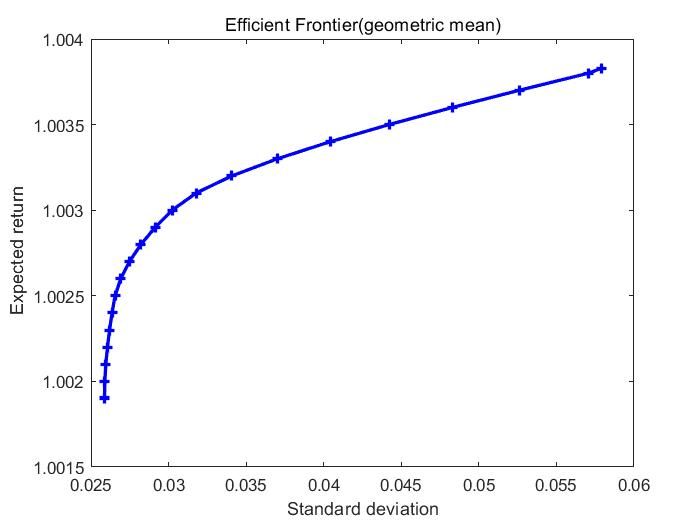
\includegraphics[width=\textwidth]{ef.jpg}
		\caption{Efficient Frontier(geometric mean)}
		\label{fig:visual_smap_o}
	\end{subfigure}
	\begin{subfigure}[b]{0.45\textwidth}
		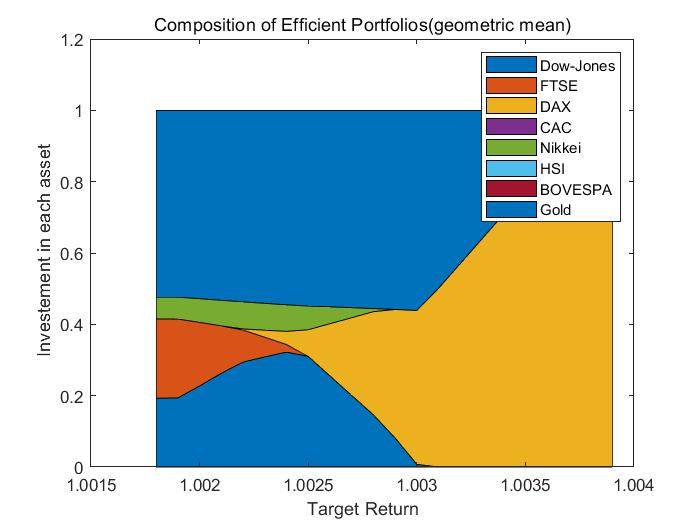
\includegraphics[width=\textwidth]{com.jpg}
		\caption{Composition of Efficient Portfolios(geometric mean)}
		\label{fig:visual_smap_k}
	\end{subfigure}
	
	\caption{}
	\label{fig:visual_smap}
\end{figure*}
The code is in appendix.\\
The optimal portfolio of the return rate $0.24\%$ is given by
$$\textbf{\textit{x}}=[0.3223, \   0.0211,   \ 0.0369, \   0, \   0.0745,  \  0,\    0, \   0.5453]$$

\textit{\textbf{4.}}\\
The optimal portfolio is given by(see code in appendix):
$$\textit{\textbf{x}}=[0.1992,\    0.0837,\    0.1345,\    0,\    0.0780,\    0,\    0,\    0.5048]$$


\textit{\textbf{5.}}\\
The standard deviation is $0.0268$.\\
The mean absolute deviation is $0.0204$.\\
The semi-deviation is $0.0188$.
\section{Appendix}
\subsection{Code of Q3}
\begin{lstlisting}
S_0_B = [1 1.3 3.56 2.49 5.07 4.11];
Scenario_0=[1.025 1.025 1.025 1.025 1.025 1.025 1.025
4 3 6 2 7 5.5 6.25;
7 9 1 5 4 6 3;
3.5 4 1 7.2 3.15 2 4.5;
6 7 2 2.5 3 8 4;
2.25 1 4 5 3 6.1 4.2];
cvx_begin
	variable y(6)
	minimize(-sum(Scenario_0'*y)/7)
	subject to 
		for i = 1:7
			Scenario_0(:,i)'*y>=0;
		end
	S_0_B*y<=0;
cvx_end
\end{lstlisting}
\subsection{Code of Q4}
Data processing
\begin{lstlisting}
clc
clear
M = csvread('indices.csv', 1, 1);
dim = size(M);
M = flip(M);
return_rate=[];
tem_return = [];
assets = {'Dow-Jones','FTSE','DAX','CAC','Nikkei','HSI','BOVESPA','Gold'};
for i =1:dim(2)
	for j = 1:(dim(1)-1)
		tem_return = [tem_return (M(j+1,i)-M(j,i))/M(j,i)];
		% Calculate the return rate
	end
	tem_return = tem_return';
	return_rate=[return_rate tem_return];
	tem_return = [];
end
return_rate = 1 + return_rate;

geo = geo_mean(return_rate);
ari = mean(return_rate);
e=[1 1 1 1 1 1 1 1];
\end{lstlisting}

\subsubsection*{Code of 4.1}
\begin{lstlisting}
Cov= cov(return_rate)*95/96;
var_Nikkei = Cov(5,5);
\end{lstlisting}
\subsubsection*{Code of 4.2}
\begin{lstlisting}
% Use geometric mean as the expected return
opt_geo=[];
expected_return_geo=[];
risk_std_geo = [];
for R=1:0.0001:1.006
	cvx_begin quiet
		variables x(8)
		minimize(x'*Cov*x)
		subject to 
			e*x==1;
			x>=0;
			geo*x >= R;
	cvx_end
	if isnan(x)
		R_largest_geo = R-0.0001;
		break
	end
	opt_geo=[opt_geo x];
	expected_return_geo=[expected_return_geo geo*x];
	risk_std_geo = [risk_std_geo sqrt(x'*Cov*x)];
end

R=1:0.0001:1.006;
diff_opt_geo = diff(opt_geo,1,2);
for i = size(diff_opt_geo,2):-1:1
	if abs(diff_opt_geo(:,i))<1e-3
		i=i+1;
		break
	end
end
R_smallest_geo = R(i);
% Get the range
i_smallest_geo=find(R==R_smallest_geo);
i_largest_geo=find(R==R_largest_geo);
\end{lstlisting}

\subsubsection*{Code of 4.3}
\begin{lstlisting}
% plot
figure;
plot(risk_std_geo(1,i_smallest_geo:end),expected_return_geo(1,i_smallest_geo:end),
'b+-','LineWidth',2);
title('Efficient Frontier(geometric mean)');
xlabel('Standard deviation');
ylabel(' Expected return');

figure;
area(R(1,i_smallest_geo:i_largest_geo),opt_geo(:,i_smallest_geo:end)')
title('Composition of Efficient Portfolios(geometric mean)');
xlabel('Target Return');
ylabel(' Investement in each asset');
legend(assets);
---------------------------------------------------
% Question 3 optimal portfolio
cvx_begin quiet
	variables x(8)
	minimize(x'*Cov*x)
	subject to 
		e*x==1;
		x>=0;
		geo*x >= 1.0024;
cvx_end
\end{lstlisting}
\subsubsection*{Code of 4.4}
\begin{lstlisting}
% Question 4
dim = size(return_rate);
mad = zeros(size(return_rate));
for i = 1:dim(1)
	mad(i,:) = (return_rate(i,:)-geo);
end
cvx_begin quiet
	variables x(8)
	minimize(ones(1,96)*abs(mad*x)/96)
	subject to
		e*x==1;
		x>=0;
		geo*x >= 1.0024;
cvx_end
optimal = x;
\end{lstlisting}
\subsubsection*{Code of 4.5}
\begin{lstlisting}
% Question 5
standard_deviation = sqrt(optimal'*Cov*optimal)
mean_absolute_deviation = mean(abs(mad*optimal))
semi_deviation = sqrt(mean(max(0,(return_rate*optimal-geo*optimal)).^2))
\end{lstlisting}
\end{document}